\section{法兰盘三视图}

{\bfseries 知识目标}
\begin{itemize}
\item 掌握回转体三视图规律
\end{itemize}

{\bfseries 技能目标}
\begin{itemize}
\item 能够应用三视图对应关系,运用AutoCAD绘制回转体的三视图
\end{itemize}

图\ref{fig:falanpanlititu}所示为工业中应用泛用于管道连接的法兰盘零件的简化形式。本任务主要是让读者了解并掌握回转体三视图表述方式,实现应用AutoCAD进行回转体类零件的三视图绘制的技能目标。
\begin{figure}[htbp]
\centering
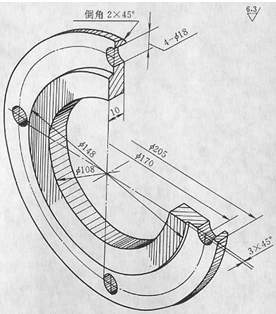
\includegraphics[scale=1]{fananlititu.png}
\caption{法兰盘}\label{fig:falanpanlititu}
\end{figure}
\subsection{绘制法兰盘主视图}
法兰盘整体是由两个圆筒叠加构成的,并具有四个用于安装的联接孔。我们先选择最能够表达的其形状的特征的方向作为其主视图。

具体绘图过程如下:

第一步:先定义图层,如图\ref{fig:falantucen}所示。
\begin{figure}[htbp]
\centering
\begin{floatrow}
\ffigbox{\caption{法兰盘图层定义}\label{fig:falantucen}}
{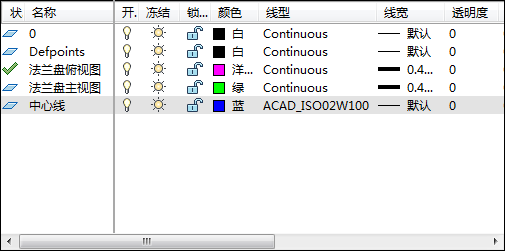
\includegraphics[scale=0.5]{falantucen.png}}
\ffigbox{\caption{法兰盘主视图}\label{fig:falanzhushitu}}{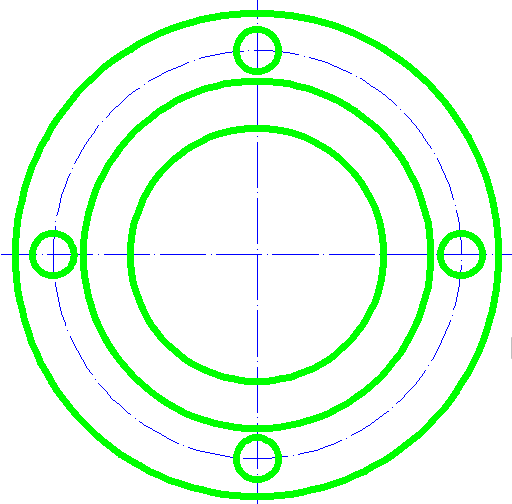
\includegraphics[scale=0.25]{falanzhushitu.png}}
\end{floatrow}
\end{figure}

第二步:绘制中心线,并完成主视图,如图\ref{fig:falanzhushitu}所示。

\begin{lstlisting}
%命令: line 指定第一点:%
%指定下一点或 [放弃(U)]: $@212<0$%
%指定下一点或 [放弃(U)]:%
%命令: LINE%
%指定第一点: @-106,106%
%指定下一点或 [放弃(U)]:$ @212<-90$%
%指定下一点或 [放弃(U)]:%
%命令: circle% 
%指定圆的圆心或 [三点(3P)/两点(2P)/切点、切点、半径(T)]: int%
%于%
%指定圆的半径或 [直径(D)]: 103%
%命令: circle %
%指定圆的圆心或 [三点(3P)/两点(2P)/切点、切点、半径(T)]: int%
%于%
%指定圆的半径或 [直径(D)]:$ <103.0000>$: 87%
%指定圆的圆心或 [三点(3P)/两点(2P)/切点、切点、半径(T)]: int%
%于%
%指定圆的半径或 [直径(D)]:$ <87.0000>$: 74%
%指定圆的圆心或 [三点(3P)/两点(2P)/切点、切点、半径(T)]: int%
%于%
%指定圆的半径或 [直径(D)]:$ <74.0000>$: 54%
%指定圆的圆心或 [三点(3P)/两点(2P)/切点、切点、半径(T)]: int%
%于%
%指定圆的半径或 [直径(D)]:$ <54.0000>$: 9%
%命令: arraypolar%
%选择对象: 找到 1 个%
%选择对象:%
%类型 = 极轴  关联 = 是%
%指定阵列的中心点或 [基点(B)/旋转轴(A)]: int%
%于%
%输入项目数或 [项目间角度(A)/表达式(E)]$ <4>:$%
%指定填充角度(+=逆时针、-=顺时针)或 [表达式(EX)] $<360>$:%
%按 Enter 键接受或 [关联(AS)/基点(B)/项目(I)/项目间角度(A)/填充%
%角度(F)/行(ROW)/层(L)/旋转项目(ROT)/退出(X)] %
%$<$退出$>$:%
\end{lstlisting}
\subsection{绘制法兰盘俯视图}
第一步:先利用长对正关系,确定定俯视图中对应部件的投影关系。
\begin{lstlisting}
%命令: line 指定第一点:%
%指定下一点或 [放弃(U)]: $ <$正交 开$>$%
%指定下一点或 [放弃(U)]:%
%命令: offset%
%当前设置: 删除源=否  图层=源  OFFSETGAPTYPE=0%
%指定偏移距离或 [通过(T)/删除(E)/图层(L)] %<%通过%>%:  10%
%选择要偏移的对象,或 [退出(E)/放弃(U)] $<$退出$>$:%
%指定要偏移的那一侧上的点,或 [退出(E)/多个(M)/放弃(U)] $<$退出$>$:%
%选择要偏移的对象,或 [退出(E)/放弃(U)] $<$退出$>$:%
%指定要偏移的那一侧上的点,或 [退出(E)/多个(M)/放弃(U)] $<$退出$>$:%
%选择要偏移的对象,或 [退出(E)/放弃(U)] $<$退出$>$:%
%命令: line %
%指定第一点: int%
%于%
%指定下一点或 [放弃(U)]: per%
%到%
%指定下一点或 [放弃(U)]:%
%命令: line %
%指定第一点: int%
%于%
%指定下一点或 [放弃(U)]: per%
%到%
%指定下一点或 [放弃(U)]:%
%命令: line %
%指定第一点: int%
%于%
%指定下一点或 [放弃(U)]: per%
%到%
%指定下一点或 [放弃(U)]:%
%命令: line %
%指定第一点: int%
%于%
%指定下一点或 [放弃(U)]: per%
%到%
%指定下一点或 [放弃(U)]:%
%命令: line %
%指定第一点: int%
%于%
%指定下一点或 [放弃(U)]: per%
%到%
%指定下一点或 [放弃(U)]:%
%命令: line %
%指定第一点: int%
%于%
%指定下一点或 [放弃(U)]: per%
%到%
%指定下一点或 [放弃(U)]:%
%命令: line %
%指定第一点: int%
%于%
%指定下一点或 [放弃(U)]: per%
%到%
%指定下一点或 [放弃(U)]:%
%命令: line %
%指定第一点: int%
%于%
%指定下一点或 [放弃(U)]: per%
%到%
%指定下一点或 [放弃(U)]:%
%命令: line %
%指定第一点: int%
%于%
%指定下一点或 [放弃(U)]: per%
%到%
%指定下一点或 [放弃(U)]:%
%命令: line %
%指定第一点: int%
%于%
%指定下一点或 [放弃(U)]: per%
%到%
%指定下一点或 [放弃(U)]:%
%命令: line %
%指定第一点: int%
%于%
%指定下一点或 [放弃(U)]: per%
%到%
%指定下一点或 [放弃(U)]:%
%命令: line %
%指定第一点: int%
%于%
%指定下一点或 [放弃(U)]: per%
%到%
%指定下一点或 [放弃(U)]:%
\end{lstlisting}

\begin{figure}[htbp]
\centering
\begin{floatrow}
\ffigbox{\caption{法兰盘俯视图}\label{fig:falanfushitu}}{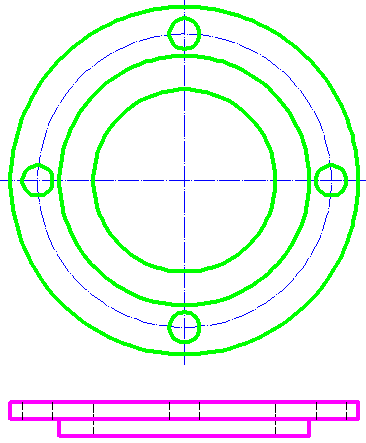
\includegraphics[scale=0.3]{falanfushitu.png}}
\ffigbox{\caption{法兰盘三视图}\label{fig:falansanshitu}}{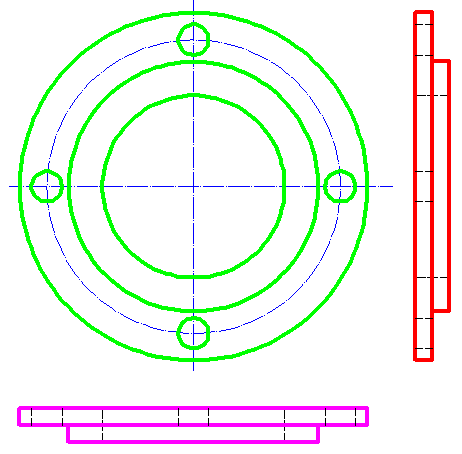
\includegraphics[scale=0.3]{falansanshitu.png}}
\end{floatrow}
\end{figure}

第二步:根据\ref{fig:falanpanlititu}所示尺寸绘出俯视图,如图\ref{fig:falanfushitu}所示。
\begin{lstlisting}
%命令: trim%
%当前设置:投影=UCS,边=无%
%选择剪切边...%
%选择对象或 $<$全部选择$>$:  找到 1 个%
%选择对象:%
%选择要修剪的对象,或按住 Shift 键选择要延伸的对象,或%
%[栏选(F)/窗交(C)/投影(P)/边(E)/删除(R)/放弃(U)]:  指定对角点:%
%选择要修剪的对象,或按住 Shift 键选择要延伸的对象,或%
%[栏选(F)/窗交(C)/投影(P)/边(E)/删除(R)/放弃(U)]:%
%命令: trim%
%当前设置:投影=UCS,边=无%
%选择剪切边...%
%选择对象或 $<$全部选择$>$:  找到 1 个%
%选择对象: 找到 1 个,总计 2 个%
%选择对象: 找到 1 个,总计 3 个%
%选择对象: 找到 1 个,总计 4 个%
%选择对象:%
%选择要修剪的对象,或按住 Shift 键选择要延伸的对象,或%
%[栏选(F)/窗交(C)/投影(P)/边(E)/删除(R)/放弃(U)]:  指定对角点:%
%选择要修剪的对象,或按住 Shift 键选择要延伸的对象,或%
%[栏选(F)/窗交(C)/投影(P)/边(E)/删除(R)/放弃(U)]:  指定对角点:%
%选择要修剪的对象,或按住 Shift 键选择要延伸的对象,或%
%[栏选(F)/窗交(C)/投影(P)/边(E)/删除(R)/放弃(U)]:%
%命令: TRIM%
%当前设置:投影=UCS,边=无%
%选择剪切边...%
%选择对象或 $<$全部选择$>$:  找到 1 个%
%选择对象:%
%选择要修剪的对象,或按住 Shift 键选择要延伸的对象,或%
%[栏选(F)/窗交(C)/投影(P)/边(E)/删除(R)/放弃(U)]:%
%选择要修剪的对象,或按住 Shift 键选择要延伸的对象,或%
%[栏选(F)/窗交(C)/投影(P)/边(E)/删除(R)/放弃(U)]:%
%选择要修剪的对象,或按住 Shift 键选择要延伸的对象,或%
%[栏选(F)/窗交(C)/投影(P)/边(E)/删除(R)/放弃(U)]:%
\end{lstlisting}

\subsection{绘制法兰盘左视图}
利用主、左高平齐,俯左宽相等的对应关系绘制左视图的相关部分,最终形成三视图如图\ref{fig:falansanshitu}所示。
\begin{lstlisting}
%命令: line 指定第一点:%
%指定下一点或 [放弃(U)]: $ <$正交 开$>$%
%指定下一点或 [放弃(U)]:%
%命令: offset%
%当前设置: 删除源=否  图层=源  OFFSETGAPTYPE=0%
%指定偏移距离或 [通过(T)/删除(E)/图层(L)] $<10.0000>$:  int%
%于  指定第二点: int%
%于%
%选择要偏移的对象,或 [退出(E)/放弃(U)] $<$退出$>$:%
%指定要偏移的那一侧上的点,或 [退出(E)/多个(M)/放弃(U)] $<$退出$>$:%
%选择要偏移的对象,或 [退出(E)/放弃(U)] $<$退出$>$:%
%命令: offset%
%当前设置: 删除源=否  图层=源  OFFSETGAPTYPE=0%
%指定偏移距离或 [通过(T)/删除(E)/图层(L)]$ <10.0000>$:  int%
%于  指定第二点: int%
%于%
%选择要偏移的对象,或 [退出(E)/放弃(U)] $<$退出$>$:%
%指定要偏移的那一侧上的点,或 [退出(E)/多个(M)/放弃(U)] $<$退出$>$:%
%选择要偏移的对象,或 [退出(E)/放弃(U)] $<$退出$>$:%
%命令: line %
%指定第一点: int%
%于%
%指定下一点或 [放弃(U)]: per%
%到%
%指定下一点或 [放弃(U)]:%
%命令: line %
%指定第一点: int%
%于%
%指定下一点或 [放弃(U)]: per%
%到%
%指定下一点或 [放弃(U)]:%
%命令: line %
%指定第一点: int%
%于%
%指定下一点或 [放弃(U)]: per%
%到%
%指定下一点或 [放弃(U)]:%
%命令: line %
%指定第一点: int%
%于%
%指定下一点或 [放弃(U)]: per%
%到%
%指定下一点或 [放弃(U)]:%
%命令: line %
%指定第一点: int%
%于%
%指定下一点或 [放弃(U)]: per%
%到%
%指定下一点或 [放弃(U)]:%
%命令: line %
%指定第一点: int%
%于%
%指定下一点或 [放弃(U)]: per%
%到%
%指定下一点或 [放弃(U)]:%
%命令: line %
%指定第一点: int%
%于%
%指定下一点或 [放弃(U)]: per%
%到%
%指定下一点或 [放弃(U)]:%
%命令: line %
%指定第一点: int%
%于%
%指定下一点或 [放弃(U)]: per%
%到%
%指定下一点或 [放弃(U)]:%
%命令: line %
%指定第一点: int%
%于%
%指定下一点或 [放弃(U)]: per%
%到%
%指定下一点或 [放弃(U)]:%
%命令: line %
%指定第一点: int%
%于%
%指定下一点或 [放弃(U)]: per%
%到%
%指定下一点或 [放弃(U)]:%
%命令: line %
%指定第一点: int%
%于%
%指定下一点或 [放弃(U)]: per%
%到%
%指定下一点或 [放弃(U)]:%
%命令: line %
%指定第一点: int%
%于%
%指定下一点或 [放弃(U)]: per%
%到%
%指定下一点或 [放弃(U)]:%
%命令: trim%
%当前设置:投影=UCS,边=无%
%选择剪切边...%
%选择对象或 $<$全部选择$>$:  找到 1 个%
%选择对象:%
%选择要修剪的对象,或按住 Shift 键选择要延伸的对象,或%
%[栏选(F)/窗交(C)/投影(P)/边(E)/删除(R)/放弃(U)]:  指定对角点:%
%选择要修剪的对象,或按住 Shift 键选择要延伸的对象,或%
%[栏选(F)/窗交(C)/投影(P)/边(E)/删除(R)/放弃(U)]:%
%命令: trim%
%当前设置:投影=UCS,边=无%
%选择剪切边...%
%选择对象或 $<$全部选择$>$:  找到 1 个%
%选择对象: 找到 1 个,总计 2 个%
%选择对象: 找到 1 个,总计 3 个%
%选择对象: 找到 1 个,总计 4 个%
%选择对象:%
%选择要修剪的对象,或按住 Shift 键选择要延伸的对象,或%
%[栏选(F)/窗交(C)/投影(P)/边(E)/删除(R)/放弃(U)]:  指定对角点:%
%选择要修剪的对象,或按住 Shift 键选择要延伸的对象,或%
%[栏选(F)/窗交(C)/投影(P)/边(E)/删除(R)/放弃(U)]:  指定对角点:%
%选择要修剪的对象,或按住 Shift 键选择要延伸的对象,或%
%[栏选(F)/窗交(C)/投影(P)/边(E)/删除(R)/放弃(U)]:%
%命令: TRIM%
%当前设置:投影=UCS,边=无%
%选择剪切边...%
%选择对象或 $<$全部选择$>$:  找到 1 个%
%选择对象:%
%选择要修剪的对象,或按住 Shift 键选择要延伸的对象,或%
%[栏选(F)/窗交(C)/投影(P)/边(E)/删除(R)/放弃(U)]:%
%选择要修剪的对象,或按住 Shift 键选择要延伸的对象,或%
%[栏选(F)/窗交(C)/投影(P)/边(E)/删除(R)/放弃(U)]:%
%选择要修剪的对象,或按住 Shift 键选择要延伸的对象,或%
%[栏选(F)/窗交(C)/投影(P)/边(E)/删除(R)/放弃(U)]:%
\end{lstlisting}
\endinput